\chapter{Background} \label{cha:background}

% The background section of the report should set the project into context by relating it to existing published work which you read at the start of the project when your approach and methods were being considered. There are usually many ways of solving a given problem, and you shouldn't just pick one at random. Describe and evaluate as many alternative approaches as possible. The published work may be in the form of research papers found in the academic literature, articles, text books, technical manuals, or even existing software or hardware of which you have had hands-on experience. Your must acknowledge the sources of your inspiration. You are expected to have seen and thought about other people's ideas; your contribution will be putting them into practice in some other context. However, avoid plagiarism: if you take another person's work as your own and do not cite your sources of information/inspiration you are being dishonest. When referring to other pieces of work, cite the sources where they are referred to or used, rather than just listing them at the end. Accidental plagiarism or not knowing how to cite and reference is not a valid reason for plagiarism. Make sure you read and digest the Department's plagiarism document .

% In writing the Background chapter you must demonstrate your ability to analyse, synthesise and apply critical judgement. Analysis is shown by explaining how the proposed solution operates in your own words as well as its benefits and consequences. Synthesis is shown through the organisation of your Related Work section and through identifying and generalising common aspects across different solutions. Critical judgement is shown by discussing the limitations of the solutions proposed both in terms of their disadvantages and limits of applicability.

In this chapter, we provide the necessary preliminary concepts to understand the problem domain and current state-of-the art in image generation.
We assume that the reader has prior knowledge of the basic concepts around artificial neural networks and their training.

\section{Diabetic Retinopathy} \label{background:classifyingdr}

Diabetic retinopathy is damage to the blood vessels of the retina caused by high blood sugar levels.
The level of damage, and hence the stage of DR, can be determined by identifying and categorising different types of lesions on the patient's retina.
A description of the appearance of major lesion types is given as follows \cite{taylor2012handbook}:
\begin{description}
    \item[Microaneurysms (MA)] \hfill \\ Small red round dots caused by weakness in the vessel's walls.
    \item[Haemorrhages (HE)] \hfill \\ Larger spots on the retina.
    \item[Hard exudates (EX)] \hfill \\ Bright yellow spots caused by the leakage of plasma.
    \item[Soft exudates (SE)] \hfill \\ White spots caused by swelling of nerve fibre. Also known as ``cotton wool spots''.
    \item[Intraretinal microvascular abnormalities (IRMA)] \hfill \\ Abnormally shaped blood vessels. Usually a precursor to neovascularization.
    \item[Neovascularization (NV)] \hfill \\ Abnormal growth of new blood vessels. Similar in appearance to IRMA, but tend to be finer and show signs of blood leakage.
\end{description}
Examples of each type of lesion, and the optic disc, are labelled on a colour fundus photograph in \Cref{fig:lesions}.
Note that, while other imaging techniques such as fluorescein angiography or optical coherence tomography (OCT) are possible, we are interested in only colour fundus photographs. 
They are key in scaling DR screening, being low-cost, easy to obtain, and offering the option of a remote ophthalmologist examination via a telemedicine platform \cite{pmid25949070}.
\begin{figure}
    \centering
    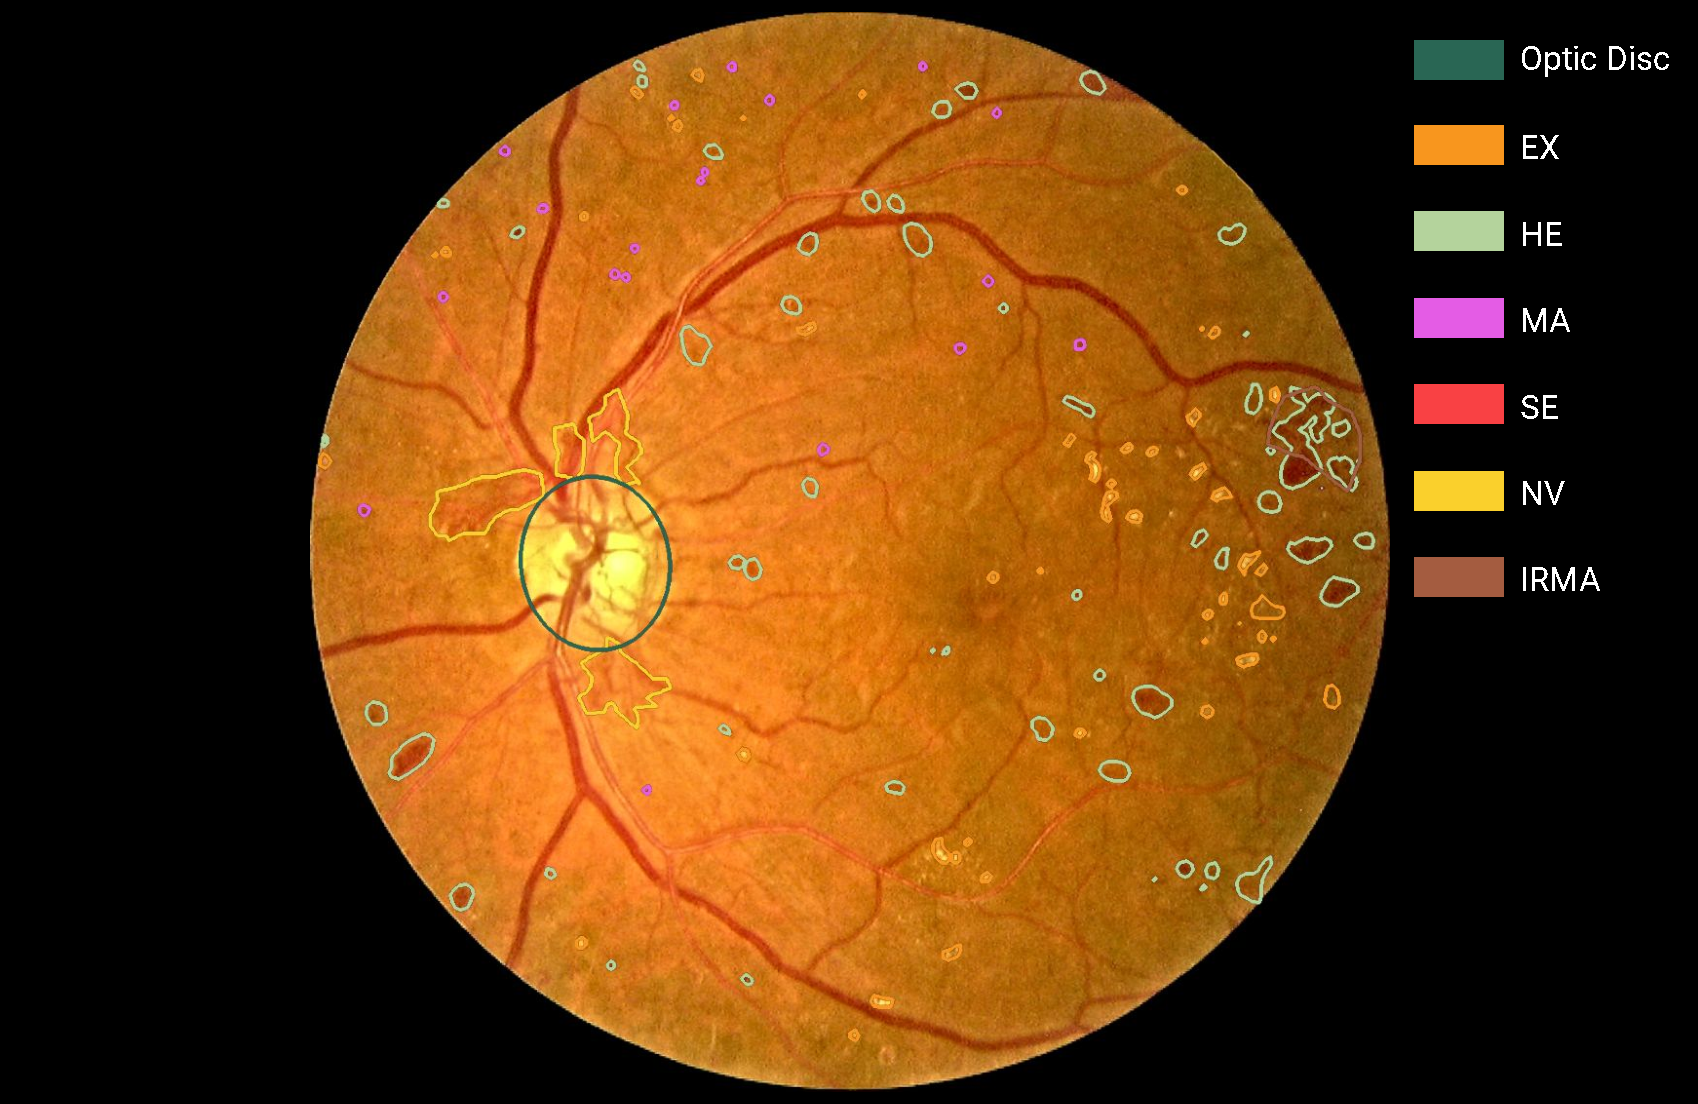
\includegraphics[width=\linewidth]{background/figs/retina.pdf}
    \caption{A retinal fundus image annotated with the optic disc as well as six types of lesions: hard exudates (EX), haemorrhages (HE), microaneurysms (MA), soft exudates (SE), neovascularization (NV), and intraretinal microvascular abnormalities (IRMA).}
    \label{fig:lesions}
\end{figure}
At the intersection of machine learning and DR detection there are a number of distinct, but related, research areas:
\begin{description}
    \item[Image-Level Grading] \hfill \\ To identify a DR severity grade for a fundus photograph. This can be according to the the international disease scale (summarised in \Cref{tab:dr_stages}), or a more coarse scale which combines several stages e.g. healthy, referred, diseased. For example, see \cite{Gulshan2016}. This task is difficult due to inter- and intra-grader variation, which causes datasets to be noisy.
    \item[Pixel-Level Segmentation] \hfill \\ To perform semantic segmentation of the retinal structure (blood vessels, optic disc) and/or lesions. For example, see \cite{Xiao_2019}.
    \item[Computer-Assisted Diagnosis] \hfill \\ To generate attention maps for suspicious areas, to be reviewed by a ophthalmologist. For example, see \cite{Wang2017}.
    \item[Image Synthesis] \hfill \\ To generate synthetic retinal fundus photographs. These could be conditioned on, for example, vascular structure or DR grade. This task is the subject of this project, and related work is discussed in greater detail in later sections.
\end{description}
\begin{table}[h]
    \centering
    \begin{tabular}{ll}
        \toprule
        Severity & Characteristics \\
        \midrule
        No apparent retinopathy & No abnormalities \\
        Mild NPDR & Microaneurysms only \\
        Moderate NPDR & More than just microaneurysms but less than severe NPDR \\
        Severe NPDR & Any of the following and no signs of PDR: \\ 
        & \tabitem > 20 intraretinal haemorrhages in all 4 quadrants \\
        & \tabitem Venous beading in $\geq$ 2 quadrants\\
        & \tabitem Intraretinal microvascular abnormalities in $\geq$ 1 quadrant \\
        PDR & One or both of: \\
        & \tabitem Neovascularisation \\
        & \tabitem Vitreous/preretinal haemorrhage \\
        \bottomrule
    \end{tabular}
    \caption{The International Clinical Diabetic Retinopathy Disease Scale \cite{ophthalmoscopy2002international}. \\ NPDR = non-proliferative diabetic retinopathy; PDR = proliferative diabetic retinopathy.}
    \label{tab:dr_stages}
\end{table}

\section{Generative Adversarial Networks} \label{sec:gans}

A Generative Adversarial Network (GAN) is a machine learning framework introduced by \citeauthor{gan} in \citeyear{gan} \cite{gan} consisting of two neural networks in adversarial competition. The generative model $G$ creates candidate images that look as ``real'' as possible, while the discriminative model $D$ attempts to distinguish between real and synthetic images. Training continues until the discriminator can no longer tell which inputs are fabricated by $G$ and which are real. In this sense, $G$ and $D$ are trained \emph{adversarially}. From this, we can derive the adversarial loss function by taking the cross-entropy of the real and generated samples:
\begin{align} \label{eq:ganloss}
    \mathcal{L}_{GAN} = \mathbb{E}_x[\log D(x)] + \mathbb{E}_z[\log (1-D(G(z))]
\end{align}
This yields the corresponding objective function:
\begin{align}
    \min_G \max_D \mathcal{L}_{GAN}
\end{align}
where $D(x)$ is the discriminator's estimate that $x \sim p_{data}$ is real; $G(z)$ is the generator's output when given random noise $z\sim p_z$; and $D(G(z))$ is the discriminator's estimate that a fake instance is real.
The discriminator will attempt to maximise this loss, whilst the generator attempts to minimise it.
In practice, this happens in alternating phases, keeping the generator fixed when updating the discriminator, and vice versa.
This means that the discriminator and generator can have differing loss functions instead of strictly adhering to the joint definition in \Cref{eq:ganloss}.

The versatility of GANs has enabled them to be applied to a plethora of problems including semantic segmentation and text generation, but their first and primary use is image synthesis.
The vanilla GAN design is far from perfect, however, and as such there has been an explosion of GAN variants since their initial introduction, making incremental improvements over each other.
In the following sections, we examine a selection of extensions and variants that are relevant to this project. 

Note that, while I have attempted to disentangle developments in GAN research over time by introducing these concepts in a coherent order, research does not always progress in a straight line, and new techniques do not always incorporate all the ideas of previous techniques.
Refer to \Cref{fig:conceptmap} for a holistic overview of how the discussed concepts relate to each other.

\begin{figure}
    \centering
    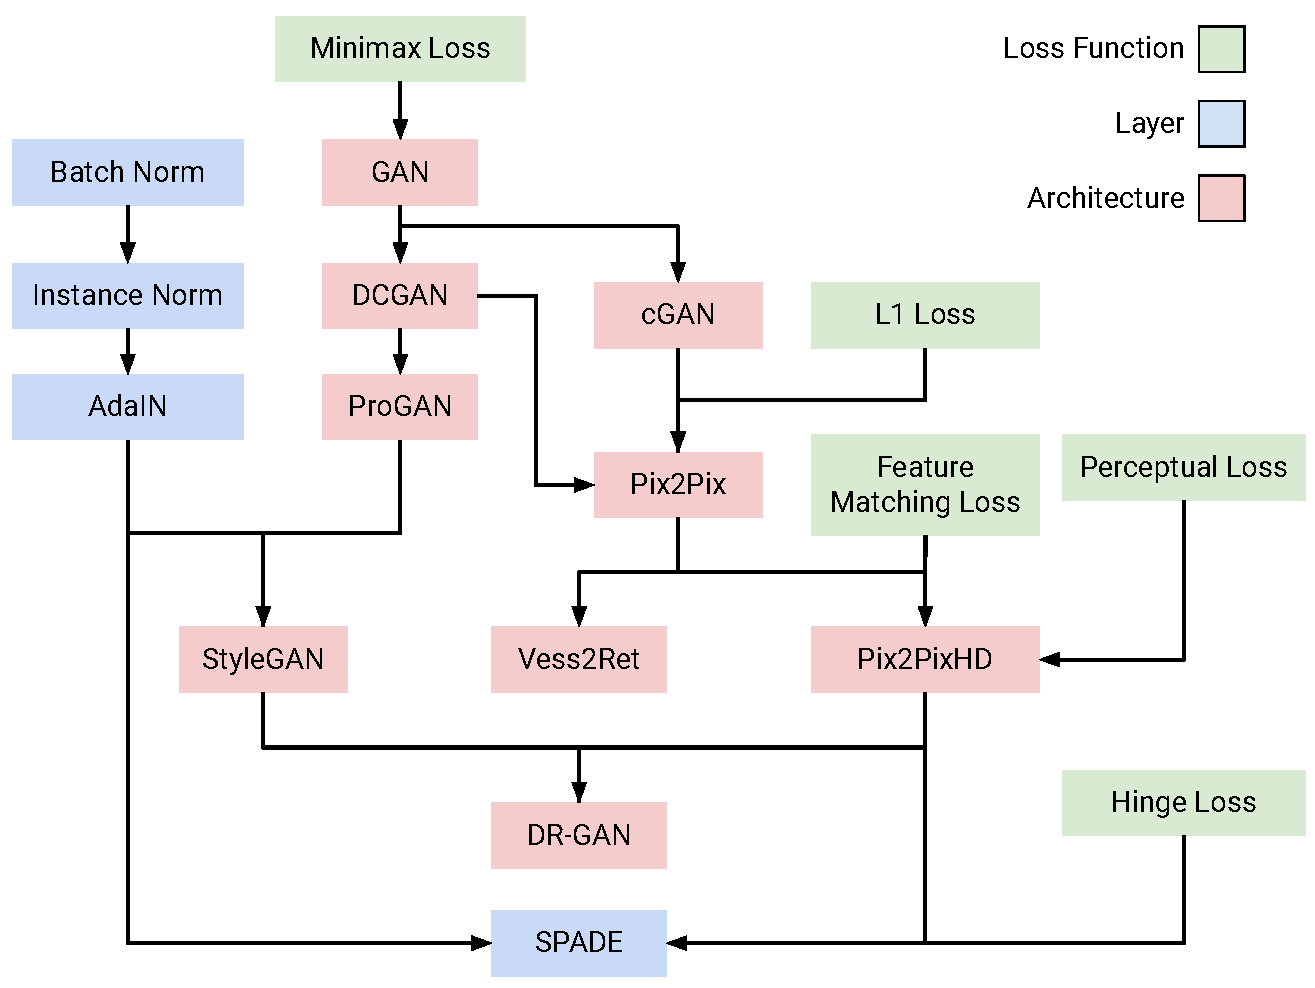
\includegraphics[width=0.6\textwidth]{background/figs/concept-map.pdf}
    \caption{Concept map of discussed techniques and how they relate to one another.}
    \label{fig:conceptmap}
\end{figure}

\section{Improving GAN Training}

Training GANs is known to be unstable, difficult to make converge, and prone to issues like mode collapse.
There have been a number of attempts to address these problems. 

\subsection{Modified Minimax Loss}

In their original paper, \citeauthor{gan} describe an issue with the original loss formulation where $G$ fails to gain any traction in the early stages of training, and therefore never even begins to converge.
This is due to $D$ being able to easily reject to the output of $G$, which causes the gradients to be extremely small.
To mitigate this, the authors propose to maximise $\log D(G(z))$ instead of minimising $\log(1-D(G(z))$ as in \Cref{eq:ganloss} i.e. the generator loss (denoted by superscript $G$) becomes
\begin{align}
    \mathcal{L}_{MM}^G = - D(G(z))
\end{align}
However, even this loss function is prone to vanishing gradients, and as a result other types of adversarial losses such as Wasserstein and Hinge loss have also been proposed.
These alternatives aim to provide consistently strong gradients throughout training.

\subsection{Feature Matching Loss} \label{sec:featurematching}

Even with the above modification, GANs can still fail to converge (i.e. the generator and discriminator fail to reach a Nash equilibrium).
This is because when the one network gets closer to the equilibrium, it can cause the other to move further from the equilibrium.
This oscillation can increase over time, causing divergence.
To address this, in \citeyear{salimans2016} \citeauthor{salimans2016} proposed a modification to the loss function called the feature matching loss \cite{salimans2016}.
In this scheme, instead of asking the generator to directly match the output of the discriminator, we ask it only to match some statistic of the real data.
These statistics are retrieved from an intermediate layer, $i$, of the discriminator, denoted by $D^{(i)}$:
\begin{align} \label{eq:fmloss}
    \mathcal{L}_{FM}^G = \left\lVert \mathbb{E}_x [ D^{(i)}(x)] - \mathbb{E}_z [D^{(i)}(G(z))] \right\rVert
\end{align}
where $\lVert \cdot \rVert$ is some norm, usually $L_1$ or $L_2$.

\subsection{Perceptual Loss}

Perceptual loss\footnote{This has also been called the ``content representation loss'' \cite{Gatys2016} and ``feature reconstruction loss \cite{johnson2016} in the literature.}, closely related to feature matching loss\footnote{The distinction between feature matching and perceptual losses is not entirely clear, with some publications even using terms interchangeably \cite{chen2017}. Here, we will use ``feature matching loss'' to refer to \Cref{eq:fmloss} and ``perceptual loss'' to refer to \Cref{eq:perceptualloss}.}, refers to the idea of defining a loss function in terms of a separate network $F$ in which image features are encoded \cite{Dosovitskiy2016}.
We take the loss as the distance between the two feature representations.
\begin{align} \label{eq:perceptualloss}
    \mathcal{L}_{P}^G = \left\lVert  F^{(i)}(x) - F^{(i)}(G(z)) \right\rVert
\end{align}
It has been shown that, in convolutional neural networks, perceptual losses measure the similarity of images in a more robust manner compared to per-pixel losses \cite{johnson2016}. 
A popular choice for network $F$, called the perceptual network, is VGG.

\subsection{Batch Normalisation} \label{sec:batchnorm}

During training, the distribution of the inputs into any given layer will constantly be changing as the parameters of preceding layers change -- a phenomenon known as ``internal covariate shift''.
This means that the current layer must keep readjusting to ever-changing distributions.
With deeper neural networks, this effect is amplified as changes in scale propagate down the layers.
Therefore, in order to keep training stable it is necessary to use lower learning rates, causing training to be slow overall.
To address this, \citeauthor{batchnorm} proposed a method called batch normalisation\footnote{While batch normalisation has been shown to be empirically effective, it has since been argued that the ``internal covariate shift'' explanation does not hold water \cite{lipton2018troubling, santurkar2019does}.}.
When applied to a particular layer, the input of said layer is re-centred (to zero mean) and re-scaled (to unit standard deviation) across the batch and spatial dimensions for each channel \cite{batchnorm}.
This allows for the use of larger learning rates since we do not run the risk of exploding gradients, which in turn enables faster training overall.

This normalising step means that the layer's activations will be unaffected by changes in scale in previous layers.
However, the authors point out that by normalising a layer we may change what the layer is capable of representing. 
To restore the ``representational power'' of the layer, we now \emph{denormalise} the normalised activations by performing an affine transformation using learned parameters. Note how this transformation is still independent of the distribution of activations in previous layers.

Formally, consider a batch of feature maps $X \in \mathbb{R}^{N\times C\times H\times W}$.
We can compute the mean and standard deviation for each channel $c$ as
\begin{align}
    \mu_c(X) &= \frac{1}{NHW} \sum_{n=1}^N \sum_{h=1}^H \sum_{w=1}^W X_{nchw} \label{eq:bnmean} \\ 
    \sigma_c(X) &= \sqrt{\frac{1}{NHW} \sum_{n=1}^N \sum_{h=1}^H \sum_{w=1}^W \left(X_{nchw}-\mu_c(X)\right)^2} \label{eq:bnstd}
\end{align}
Then the batch transform for each element is given by
\begin{align}
    \text{BN}_{\gamma, \beta}(X_{nchw}) = \gamma_c \left( \frac{X_{nchw}- \mu_c(X)}{\sigma_c(X)}\right) + \beta_c
\end{align}
where $\gamma, \beta \in \mathbb{R}^C$ are the per-channel transformation parameters.

\section{Image Synthesis}

This section establishes variations on GANs that establish the current state-of-the-art in image synthesis.

\subsection{Hierarchical GANs} \label{sec:hierarchgan}

The original paper detailing GANs by \citeauthor{gan} uses the MNIST dataset as a demonstration of the capability of GANs.
These images are very low-resolution, at just $28\times 28$ pixels, due to the fact that the original approach did not scale well to high-resolution images.

In classical computer vision, the concept of a Laplacian pyramid on which filters can operate on multiple different scales is well established \cite{1095851}. Extending this idea to GANs, one of the first attempts at improving high-resolution image synthesis was LAPGAN, introduced by \citeauthor{DBLP:journals/corr/DentonCSF15} in 2015 \cite{DBLP:journals/corr/DentonCSF15}, where a separate generative CNN is trained at each scale. 
Since then, variants on this key insight of ``stacking'' models that operate on different scales has been explored thoroughly, whether it is stacking entire GANs \cite{DBLP:journals/corr/HuangLPHB16}, stacking only discriminators \cite{TCWang2017}, or stacking only generators \cite{DBLP:journals/corr/GhoshKNTD17}. 

In spite of these advances, high-resolution image synthesis has remained difficult due to the fundamental fact that the increased detail makes it easier for the discriminator to distinguish real from generated images, amplifying the vanishing gradient problem that has historically plagued GAN training. 

\subsection{DCGAN}

The difficulty of scaling up a GAN with CNNs to generate high-resolution images led to LAPGAN's alternative approach of leveraging multiple separate CNNs.
Deep Convolutional GANs (DCGAN) are a class of GAN architectures proposed by \citeauthor{dcgan} in \citeyear{dcgan} \cite{dcgan}.
In their paper, the authors outline a set of constraints that should be adhered to in order to create GANs which can produce higher-resolution images, and whose training is more stable.
\begin{itemize}
    \item Use strided convolutions in the discriminator and fractional-strided convolutions in the generator instead of pooling layers.
    \item Use batch normalisation in the generator and discriminator.
    \item Remove fully-connected layers.
    \item Use ReLU activation for all layers in the generator, except the output which should use $\tanh$.
    \item Use leaky ReLU activation for all layers in the discriminator.
\end{itemize}

\subsection{Progressive Growing GAN}

Building on these ideas, progressive growing GANs (ProGAN) were introduced by \citeauthor{DBLP:journals/corr/abs-1710-10196} in \citeyear{DBLP:journals/corr/abs-1710-10196} \cite{DBLP:journals/corr/abs-1710-10196}.
The fundamental idea is that instead of training all layers at once, we incrementally \emph{grow} both the discriminator and generator during training, starting from low-resolution images up to high-resolution images.
With each additional layer that is faded in, finer details at higher resolutions are able to be added.
This allows for the stable training of generator models that are capable of producing high-quality images.

\subsection{Instance Normalisation} 

Instance normalisation is similar in concept to batch normalisation, but we just normalise the inputs across the only the spatial dimensions for each sample \emph{and} channel.
Although batch normalisation was introduced with the intention of improving the rate of training, in \citeyear{instancenorm} \citeauthor{instancenorm} found that just by replacing batch normalisation with instance normalisation, the \emph{visual quality} of certain image synthesis networks could be significantly improved \cite{instancenorm}.

Consider, as in \Cref{sec:batchnorm}, a batch of feature maps $X\in \mathbb{R}^{N \times C \times H \times W}$.
We can compute the mean $\mu_{nc}$ and standard deviation $\sigma_{nc}$ for each sample and channel as
\begin{align}
    \mu_{nc}(X) &= \frac{1}{HW} \sum_{h=1}^{H} \sum_{w=1}^W X_{nchw} \\
    \sigma_{nc} &= \sqrt{\frac{1}{HW} \sum_{h=1}^H \sum_{w=1}^W \left(X_{nchw}-\mu_{nc}(X)\right)^2}
\end{align}
Note the differences between this and the definitions used in batch normalisation (\Cref{eq:bnmean} and \eqref{eq:bnstd}). Then the instance normalisation transform for each element is given by
\begin{align}
    \text{IN}_{\gamma, \beta}(X) = \gamma_c \left( \frac{X_{nchw} - \mu_{nc}(X)}{\sigma_{nc}(X)} \right) + \beta_c
\end{align}
where $\gamma, \beta \in \mathbb{R}^C$ are the per-channel transformation parameters.

\subsection{AdaIN} \label{sec:adain}

Adaptive Instance Normalisation (AdaIN) is a conditional extension to instance normalisation introduced in \citeyear{adain} by \citeauthor{adain} \cite{adain}, meaning that it uses external information to learn the denormalisation parameters $\gamma, \beta$.
In contrast, standard instance normalisation and batch normalisation are unconditional normalisation layers.
AdaIN takes a content input $X$ and an adaptive style input $Y$, and aligns the mean and variance of $X$ with those of $Y$.
Unlike batch normalisation or instance normalisation, its parameters are not learned but instead adaptively computed from $Y$.
\begin{align}
    \text{AdaIN} (X, Y) = \sigma_{nc}(Y) \left( \frac{X_{nchw} - \mu_{nc}(X)}{\sigma_{nc}(X)} \right) + \mu_{nc}(Y)
\end{align}
Intuitively, we can understand this operation as applying the style of $Y$ to $X$. Despite being first developed for style transfer, AdaIN was later adapted for a variety of other computer vision tasks.

\subsection{StyleGAN} \label{sec:stylegan}

\begin{figure}[h]
    \centering
    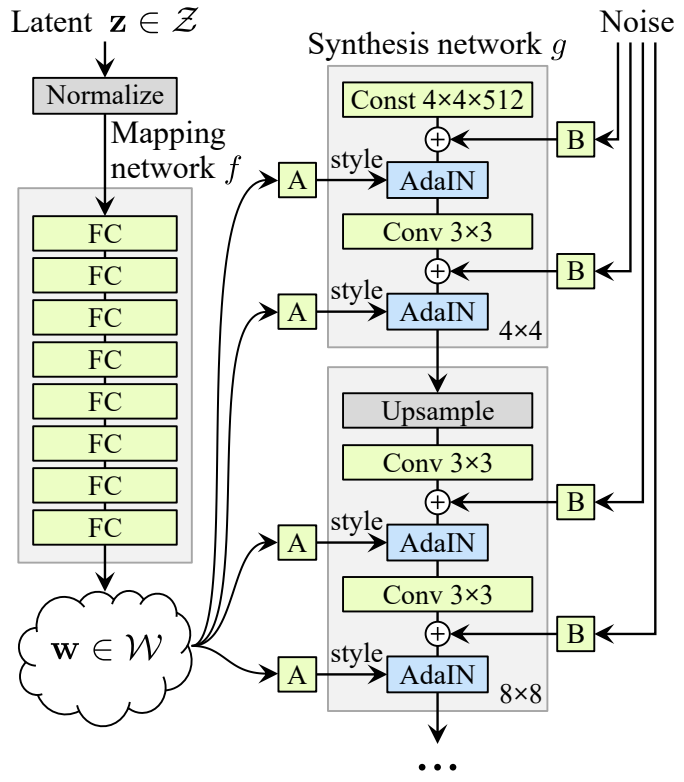
\includegraphics[width=0.5\textwidth]{background/figs/stylegan.png}
    \caption{Diagram of the StyleGAN generator architecture. Taken from \cite{stylegan}.}
    \label{fig:styleganarch}
\end{figure}

Introduced in \citeyear{stylegan} by \citeauthor{stylegan}, StyleGAN combines both AdaIN and progressive growing to produce high-resolution photo-realistic images.
Up until now, we have been providing a linear, feed-forward neural network generator a latent code $z \in \mathcal{Z}$ at the input layer.
Instead, StyleGAN introduces a generator architecture in which a vector in the intermediate latent space $w \in \mathcal{W}$ is supplied to AdaIN layers after each convolutional layer.
\Cref{fig:styleganarch} shows this new architecture and the role of the mapping network.
The intermediate latent space $\mathcal{W}$ is learned by a mapping network, and the point in the network at which provide $w$ is provided is correlated with how coarse or fine the transferred features are.

\section{Conditional Image Generation}

Having discussed the progression of \emph{unconditional} high-resolution image generation, we now turn to work done in the field of \emph{conditional} image generation. 
We start by looking at how GANs can be guided to generate images of a certain class, and then at the specific task of image-to-image synthesis, wherein an input image (such as a semantic label map) is transformed to an output image (such as a retinal fundus image). 

\subsection{Conditional GAN}

One of the earliest extensions to the original design, a conditional GAN (cGAN) extends the vanilla GAN by conditioning on additional information $y$, allowing us to direct the generation process \cite{DBLP:journals/corr/MirzaO14}.
Consequently, the loss function previously defined in \Cref{eq:ganloss} now becomes
\begin{align} \label{eq:cganloss}
    \mathcal{L}_{cGAN} = \mathbb{E}_{x, y}[\log D(x|y)] + \mathbb{E}_{y, z}[\log (1-D(G(z|y))]
\end{align}
Today, there are four well-understood methods of conditioning the generator:
\begin{itemize}
    \item concatenation of a vector representing the label;
    \item adding an auxiliary classifier;
    \item using projection; and
    \item conditional batch normalisation.
\end{itemize}

\subsection{Pix2Pix} \label{sec:pix2pix}

In \citeyear{pix2pix}, \citeauthor{pix2pix} introduced pix2pix, a conditional GAN for general purpose image-to-image translation (as opposed to class-conditional image generation), capable of producing photo-realistic images from a semantic label map \cite{pix2pix}.
First, inspired by \cite{DBLP:journals/corr/PathakKDDE16}, the authors added a global reconstruction loss penalty to the basic adversarial cGAN objective (\Cref{eq:cganloss}), implemented using the $L_1$ norm.
\begin{align}
    \mathcal{L}_{L_1} = \mathbb{E}_{x, y, z} \left\lVert x - G(z|y) \right\rVert_1
\end{align}
This captures the overall structure of the image, and therefore serves to prevent the generator from creating synthetic images that deviate too far from the real image. 
Together, this yields the overall objective function
\begin{align} \label{eq:pix2pixloss}
    \mathcal{L}_{pix2pix} = \mathcal{L}_{cGAN}(G, D) + \lambda \mathcal{L}_{L_1}(G)
\end{align}
where $\lambda$ is a hyperparameter that balances the contribution of the two terms.

Next, they iterate on the DCGAN generator and discriminator architectures. For the generator, skip-connections are added to the standard encoder-decoder architecture, resembling that of a U-Net \cite{unet}, used to directly share information across the network.
Turning to the discriminator, the authors identified that since the $L_1$ loss from above already enforces correctness at the larger scale, the discriminator need only penalise at smaller scales.
For this reason, they opted for a patch-based CNN discriminator which calculates loss for $N\times N$ patches, where $N$ is smaller than the image size.

\subsection{Pix2PixHD}

While promising, pix2pix was only designed to generate images at resolutions up to $512\times 512$.
Attempting to apply pix2pix to higher resolution images resulted in unstable training, and blurry details in the generated images.
To address these issues, in \citeyear{pix2pixhd} \citeauthor{pix2pixhd} released pix2pixHD \cite{pix2pixhd} as an extension to pix2pix. 

Building on the idea of a hierarchical GAN structure, a multi-scale generator is adopted to work on images of different resolutions.
In their paper, the authors choose to use two sub-networks with one acting as a ``global generator'' and the other a ``local enhancer''.

Similarly, multi-scale discriminators operating at three different scales are employed.
This works slightly differently to the multi-scale generators, since instead of having a nested sub-network, three separate networks are used.

The adversarial loss defined in \Cref{eq:pix2pixloss} is improved by adding a feature matching loss.
Together, we get the overall objective:
\begin{align} \label{eq:pix2pixhdloss}
    \min_G \Bigg( \bigg( \max_{D_1, D_2, D_3} \sum_{k=1, 2, 3} \mathcal{L}_{GAN} (G, D_k) \bigg) + \lambda_{FM} \sum_{k=1, 2, 3} \mathcal{L}_{FM} (G, D_k) \Bigg)
\end{align}
The discriminator's objective is maximised over each of the discriminators, and that $D_k$ does not maximimise $\mathcal{L}_{FM}$, serving only as a feature extractor. 
They also found that adding perceptual loss using a pre-trained VGG network slightly improved results, but was not critical.
With the perceptual loss, we have the objective:
\begin{equation} \label{eq:pix2pixhdloss2}
\begin{split}
    \min_G & \Bigg(\bigg( \max_{D_1, D_2, D_3} \sum_{k=1, 2, 3} \mathcal{L}_{GAN} (G, D_k) \bigg) \\
           &\quad + \lambda_{FM} \sum_{k=1, 2, 3} \mathcal{L}_{FM} (G, D_k) \\
           &\quad + \lambda_{P} \min_{D_k} \sum_{k=1, 2, 3} \mathcal{L}_{P} (G, D_k) \Bigg)
\end{split}
\end{equation}
To enhance object edges, instance boundary maps are used.

\section{Metrics}

We introduce some more uncommon metrics that the may be unfamiliar to the reader.

\subsection{Fréchet Inception Distance}

The Fréchet Inception Distance (FID) \cite{fid} is a metric for assessing the ``quality'' and diversity of generated images by comparing the distribution of the images used to train the generator with the distribution of generated images.
Specifically, feature vectors from a pre-trained Inception-v3 network \cite{inceptionv3} are used to build the distribution $\mathcal{N}(\mu, \Sigma)$ on the generated images, and the distribution $\mathcal{N}(\mu_w, \Sigma_w)$ on real images. 
Then, we calculate the FID score as the Wasserstein metric between these two distributions:
\begin{align}
    \text{FID} = \lvert \mu - \mu_w \rvert^2 + \text{tr}(\Sigma + \Sigma_w - 2(\Sigma \Sigma_w))^\frac{1}{2}
\end{align}
In essence, a smaller FID indicates a smaller distance between the two distributions.
FID is not without its issues \cite{improved_precision}, however it remains the most popular GAN evaluation metric as of today.

In this work, we use Maximilian Seitzer's PyTorch implementation of the FID score\footnote{\url{https://github.com/mseitzer/pytorch-fid}}, with feature vectors extracted from the final average pooling layer of the Inception network.

\subsection{Cohen's Quadratic Weighted Kappa}

Cohen's kappa, $\kappa$, is a metric which measures the degree of agreement between two raters who each classify $N$ items into $C$ mutually exclusive categories.
$\kappa = 1$ indicates complete agreement, $\kappa = 0$ indicates random agreement, and $\kappa < 0$ indicates worse than random agreement.
It is calculated by
\begin{align}
    \kappa = \frac{p_o - p_e}{1 - p_e}
\end{align}
where $p_o$ is the observed probability of agreement, and $p_e$ is the probability of random agreement.
We can also generalise this statistic to the weighted kappa, which is useful when some disagreements are more important than others.
In our case, we use quadratic weighting, calculated as
\begin{align}
    \kappa = 1 - \frac{\sum_{i=1}^k \sum_{j=1}^k w_{ij}x_{ij}}{\sum_{i=1}^k \sum_{j=1}^k w_{ij} m_{ij}}
\end{align}
Cohen's quadratic weighted kappa is used as the primary metric by both Kaggle DR grading competitions.

\chapter{Related Work} \label{cha:relatedwork}

We now set the research context in which to understand this project's contributions.

\section{Retinal Image Synthesis} \label{sec:retinalimagesynthesis}

% Automatic Generation of Synthetic Retinal Fundus Images (Fiorini 2014)
% Towards Adversarial Retinal Image Synthesis (Costa 2017)
% Adversarial Synthesis of Retinal Images from Vessel Trees
% End-to-End Adversarial Retinal Image Synthesis (Costa 2017)
% Unsupervised histopathology image synthesis (2017)
% Synthesizing retinal and neuronal images with generative adversarial nets (Tub-GAN) (2018)
% Retinal image synthesis from multiple-landmarks input with generative adversarial networks (2019)
% DR GAN (2020)

Early work surrounding the generation of synthetic retinal fundus images involved patch-based techniques and complex mathematical models representing the anatomy of the eye \cite{BONALDI201654, N20103:2014}.
Different algorithms had to be proposed for different components of the eye, relying heavily on domain knowledge.

\subsection{Vess2Ret}

More recently, purely data-driven approaches have been shown to be highly effective.
In \citeyear{Costa2017}, \citeauthor{Costa2017} published their foundational work utilising GANs for retinal image synthesis, dubbed vess2ret \cite{Costa2017}.
The proposed generator network operated by performing image-to-image translation from a vessel network to a retinal fundus image.
Like pix2pix, they add a global $L_1$ loss term, using \Cref{eq:pix2pixloss} as their loss function.
In the absence of a large dataset containing manual annotations, vessel masks were inferred from the output of a segmentation model.
The network architectures also resemble those of pix2pix, using a U-Net architecture for the generator and patch-based CNN for the discriminator.

However, this approach still suffers some major drawbacks. 
The fact that the generator relies on a vessel segmentation mask as input is unideal since the user will have to either (a) manually obtain their own vessel segmentation; (b) use a pre-existing vessel segmentation, of which there is a limited pool; or (c) infer a vessel segmentation (as the authors did) which may be unreliable.
Moreover, since a vessel segmentation maps to exactly one synthetic retina, data diversity is naturally limited.
The authors note that a poorly inferred vessel network, as may be produced by a segmentation model, fails to produce a usable fundus image. 
The output images have a resolution of $512 \times 512$ which, while large relative to the images often used in computer vision publications at the time, is small compared to those produced by modern fundus photography.
% \begin{figure}
%     \centering
%     \begin{subfigure}{0.3\textwidth}
%         \centering
%         \includegraphics[width=\textwidth]{example-image-a}
%         \caption{Generator architecture used in vess2ret \cite{Costa2017}.}
%         \label{fig:costa2017gen}
%     \end{subfigure}
%     \hspace{0.1\textwidth}
%     \begin{subfigure}{0.3\textwidth}
%         \centering
%         \includegraphics[width=\textwidth]{example-image-b}
%         \caption{Discriminator architecture used in vess2ret \cite{Costa2017}.}
%         \label{fig:costa2017dis}
%     \end{subfigure}
% \end{figure}

The same authors extend this existing architecture in a later work by removing the dependency on a pre-existing vessel segmentation as input \cite{Costa2018}.
Instead, an adversarial autoencoder is employed to generate vessel segmentation masks, which can be fed into the previously described image-to-image model.
This requires the user to simply supply a sample from a multivariate normal distribution, which means that a theoretically unbounded number of different vessel segmentations can be generated (although this does not speak for diversity).
While this overcomes the first of the issues with the previous work by obviating the need for the user to obtain a segmentation mask, the generated vasculatures are prone to displaying abnormalities, and the issue of resolution remains.

\subsection{Tub-GAN}

\citeauthor{tubgan} \cite{tubgan} incrementally built upon this work in \citeyear{tubgan} by introducing Tub-GAN. 
It resembles its predecessor in that the same loss function is used, and the generator architecture is also based on U-Net, except using $\tanh$ in the output layer instead of the sigmoid function.
They depart from vess2ret, however, in their discriminator design. Instead of using a patch-based CNN, a DCGAN is used, consisting of Convolution-BatchNorm-LeakyReLU blocks.
The notable improvements are the fact that manual annotations are used for training, and that the generator takes a noise code which allows for stochastic variation in the outputs from a single vessel segmentation.
However, in the absence of a vessel generator, it reinstates a dependency on a pre-existing vessel network annotation.
% \begin{figure}
%     \centering
%     \begin{subfigure}{0.3\textwidth}
%         \centering
%         \includegraphics[width=\textwidth]{example-image-a}
%         \caption{Generator architecture used in TubGAN \cite{tubgan}.}
%         \label{fig:zhao2018gen}
%     \end{subfigure}
%     \hspace{0.1\textwidth}
%     \begin{subfigure}{0.3\textwidth}
%         \centering
%         \includegraphics[width=\textwidth]{example-image-b}
%         \caption{Discriminator architecture used in TubGAN \cite{tubgan}.}
%         \label{fig:zhao2018dis}
%     \end{subfigure}
% \end{figure}

While representing an important step towards the generation of synthetic fundus images, both Tub-GAN and vess2ret lack the ability to control the generation of pathological instances.
However, in the same publication, the authors also present a variant of Tub-GAN incorporating style transfer called Tub-sGAN which presents a possible solution to this limitation.
In the Tub-sGAN framework, a target style is provided alongside the input segmentation.
The output image is expected to posses the style of the target image, while retaining the structure dictated by the segmentation.
This is much more useful since we now have the ability to transfer the texture of pathological examples onto the existing vasculature, which should include its lesions.

Nonetheless, a few shortcomings are noted.
First, the generated images still exhibit failure cases when they are not anatomically correct, particularly with respect to the optic disc and macula.
Furthermore, while the style-transfer appears to work well for global texture, it performs poorly in synthesising fine local details.
This is problematic since many retinal lesions are extremely small.
Although the authors report increased segmentation performance of vasculatures, we are interested in the more challenging task of lesion segmentation, whose ground-truths are not supplied by this network.

\subsection{Retinal Pathological Descriptor}

In 2019, \citeauthor{Niu_2019} \cite{Niu_2019} proposed an interesting ``symptom transfer'' network which allowed for lesion manipulation by exploiting the neuronal activations of an existing image-level DR grading network. 
This allows them to arbitrarily augment the position and quantity of lesions in generated images.

While interesting in concept, there is no ability to directly condition the generation on DR severity or lesion segmentations.
Therefore, we consider this work orthogonal to our objectives.

\subsection{DR-GAN}

More recently, in \citeyear{Zhou_2020}\footnote{The 2020 work is an extension of preliminary work published in 2019.
We consider the extended work only, since it supersedes the preliminary work.} \citeauthor{Zhou_2020} introduced DR-GAN \cite{Zhou_2020}: a network that ensembles many of the discussed techniques and applies them to retina generation.
DR-GAN draws heavily from recent developments in image-to-image translation by incorporating feature matching loss; multi-scale generators and discriminators; instance boundary maps; spatial and channel attention; and adaptive instance normalisation.
By leveraging these methods, DR-GAN overcomes many of the limitation of prior work, taking into account image-level grade information, pixel-wise lesion labels, and optic disc instance masks.

The authors acknowledge that, due to the extremely small size of lesions, synthesis of fundus images must be done at a high resolution to be useful.
To deal with this, they employ multi-scale generators and discriminators similar to those used in pix2pixHD. 
In order to preserve very fine features, they use a spatial and channel attention module (SCA) in the synthesis blocks inspired by \cite{sca1}, which in turn is inspired by \cite{sca2}.
Recalling the techniques used in StyleGAN, each of the synthesis blocks also contains an AdaIN layer which gives the ability to manipulate the grade of the generated images using what the authors call ``adaptive grading vectors''.
The latent grading space is first learnt using the ResNet-50 network.
From this, a set of normal distributions representing the grading space are computed.
During synthesis, the appropriate distribution is sampled from and injected into the AdaIN component of synthesis blocks.
In this way, the ``style'' of the sampled vector is transferred to the generated image. 
They extend the pix2pixHD loss function by adding a classification loss $\mathcal{L}_C$, specifically focal loss \cite{focal}, to combat class imbalance. They use VGG-19 as their perceptual network.
\begin{equation}
\begin{split}
    \min_G & \Bigg(\bigg( \max_{D_1, D_2, D_3} \sum_{k=1, 2, 3} \mathcal{L}_{GAN} (G, D_k) \bigg) \\
           &\quad + \lambda_{FM} \sum_{k=1, 2, 3} \mathcal{L}_{FM} (G, D_k) \\
           &\quad + \lambda_{P} \min_{D_k} \sum_{k=1, 2, 3} \mathcal{L}_{P} (G, D_k) \\
           &\quad + \lambda_{C} \min_{D_k} \sum_{k=1, 2, 3} \mathcal{L}_{C} (G, D_k) \Bigg)
\end{split}
\end{equation}
DR-GAN represents the state-of-the-art at the time of writing, incorporating some of the most recent techniques in computer vision.
The authors are able to demonstrate quantitatively the improvements in image quality over previous methods, and briefly show how synthetic data can improve classification performance. However, the effect of synthetic data on segmentation performance is not discussed. The model is still held back by limitations in the training data, and hence still exhibits a number of failure cases. DR-GAN still relies upon inferred structural and lesion segmentation masks to bootstrap its training due to the lack of manually annotated data. 

One concern that is unclear from the paper is how these adaptive grading vectors interact with the lesions of the input mask.
For instance, if a lesion mask exhibiting proliferative DR is given to the network, and during synthesis adaptive grading vectors corresponding to a healthy retina are provided, what will the resulting output resemble? 
And will the lesion mask still be useful if the lesions have been manipulated?
Without the source code, these questions remain unanswered.

\section{Semantic Label Generation}

Meanwhile, literature on the task of semantic label generation is relatively sparse.
\citeauthor{wang2016} \cite{wang2016} first introduced this factorisation into ``structure'' and ``texture'' in \citeyear{wang2016} when attempting to first generate normal maps which encode the geometry of the scene, and from this generating a realistic 2D image.
Their ``Structure-GAN'' generates small $72\times72\times3$ images, and the generator is deeper than the discriminator.
They also apply joint fine-tuning of both networks together, after training each one independently.

Later, in \citeyear{ghelfi2019}, \citeauthor{ghelfi2019} \cite{ghelfi2019} introduced a variant of the GAN where the last layer is simply replaced by a softmax layer.
The authors describe this as a ``more principled'' approach to generating semantic images, as opposed to treating them like standard RGB images, as in \citeauthor{wang2016}'s earlier work.
However, beyond that the papers insights into the challenges unique to this domain are limited.

More recently, in \citeyear{volokitin2020}, \citeauthor{volokitin2020} \cite{volokitin2020} went on to apply a similar technique to demonstrate how the generation of natural images could be separated into the distinct steps of layout prediction and texturing.
As opposed to improving segmentation performance, they were instead motivated by how this decomposition could improve the plausibility of multi-object scenes.
To generate semantic labels they used a DCGAN architecture, and a pix2pix model for image texturing.

Concurrently, \citeauthor{azadi2019} \cite{azadi2019} introduced a method in which the two components are trained independently at first, then fine-tuned by training in an end-to-end fashion, resembling the aforementioned Structure-GAN by \citeauthor{wang2016}.
This approach was dubbed the ``Semantic Bottleneck GAN'', or SB-GAN.
The authors note how the task of learning the interactions between structural elements to generate discrete labels is ``extremely challenging''.
However, the focus of their work was generating high-fidelity images, and did not study the effect on downstream tasks.
Moreover, the end-to-end fine-tuning was done by introducing an additional, unconditional discriminator, trained to distinguish real RGB images and those generated from synthetic layouts.
This is likely to weaken the conditioning between the semantic labels and the output image, potentially making this approach inappropriate for our use case since we would like to use the semantic labels as segmentation maps.

Moreover, none of these approaches attempt class-conditioning of semantic labels, nor do they evaluate the effect of synthetic data on downstream tasks.
A further complication is that the semantic labels of interest to us are far sparser than those used in the datasets of previous work.

\section{Training on Synthetic Data}

There already exists a history of synthetic data already being used to train machine learning models; however this work has largely been to do with using 3D scenes to train 2D computer vision algorithms (\cite{gaidon2018} provides a good overview).
Regardless, this has built a case that synthetic data could result in a real-world improvement. 
As early as \citeyear{gaidon2016}, \citeauthor{gaidon2016} \cite{gaidon2016} showed that pre-training on synthetic data and subsequent fine-tuning on real data could improve the performance of computer vision algorithms. 

Even closer to our mixed-data approach, \citeauthor{shrivastava2016} \cite{shrivastava2016} showed that training on a mixture of real and synthetic data improved performance of pose estimation models, compared to training on only real data.

